\section{Distribuzione Throughput del Cloudlet}
A seguito della validazione del modello analitico tramite l'esecuzione della
simulazione, si è provato a stimare la distribuzione del throughput del cloudlet
al variare del parametro $S$.

Dalla rappresentazione dei dati in un istogramma (figura~\ref{thrclet_hist}),
sembra emergere la forma di una distribuzione esponenziale.

\begin{figure}[!h]
\centering
%
\begin{subfigure}[t]{0.49\textwidth}
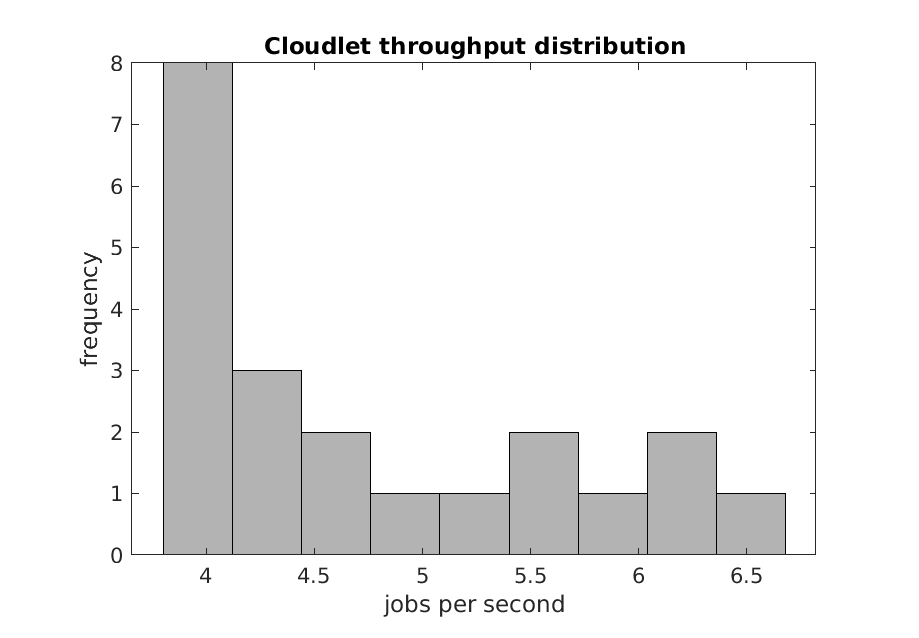
\includegraphics[width=\textwidth]{figures/thrclet_hist}
\caption{distribuzione throughput cloudlet}
\label{thrclet_hist}
\end{subfigure}
%
\begin{subfigure}[t]{0.49\textwidth}
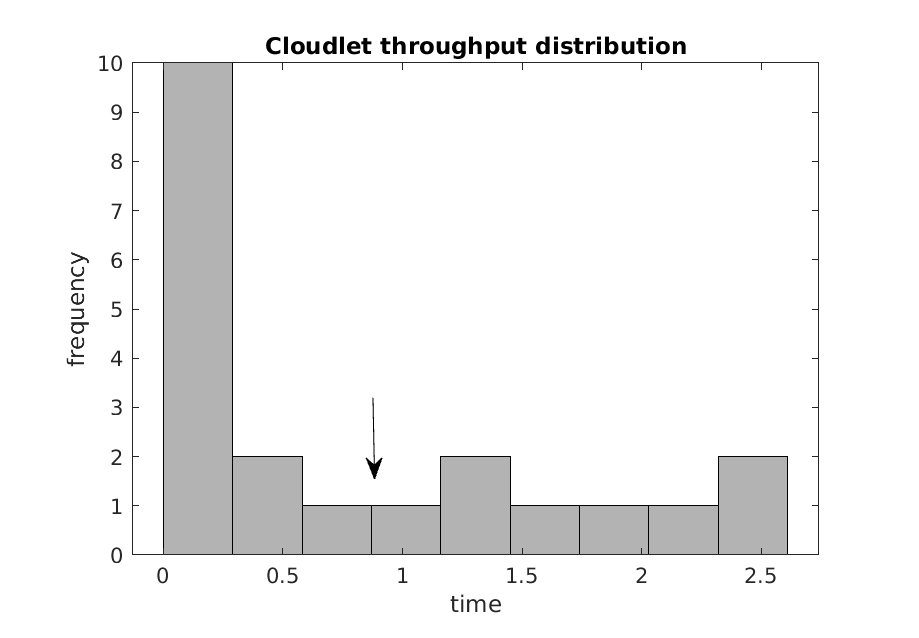
\includegraphics[width=\textwidth]{figures/thrless_hist}
\caption{Distribuzione traslata nello 0}
\label{15_intperc}
\end{subfigure}
\caption{Istogrammi distribuzione throughput del cloudlet}
%
\end{figure}

Per la proprietà di mancanza di memoria della distribuzione, è lecito traslare
il grafico in prossimità dello 0, e considerare il throughput come se fosse un
tempo di vita residuo.

La costante di decadimento $\mu$ può essere stimata, sfruttando il fatto che
dopo un tempo pari a $1/\mu$ viene meno circa il $63\%$ dell'area sottesa dal
curva che approssima la distribuzione. 
Quindi, si può stabilire tale tempo individuando il punto in cui viene
tagliata fuori la suddetta porzione di ``rettangoli'', ciò avviene in prossimità
dell'istante 1 in cui vengono lasciati a sinistra 13 unità su 21, pertanto si
può concledere che il throughput del cloudlet è approssimabile con una variabile
aleatoria esponenziale di parametro $\mu=1$.

La figura~\ref{thrclet_cdf} mostra la funzione di ripartizione della
distribuzione traslata nello 0.
\begin{figure}[!h]
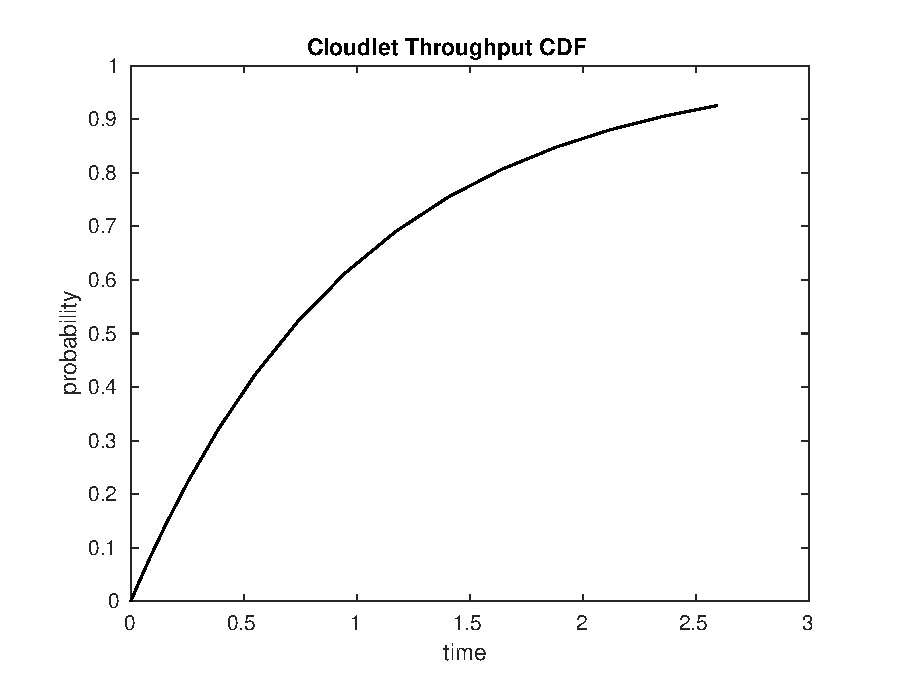
\includegraphics[width=0.7\textwidth]{figures/thrclet_cdf}
\centering
\caption{Funzione di ripartizione}
\label{thrclet_cdf}
\end{figure}
